\documentclass[compress]{beamer}

\mode<presentation>
{
  %\usetheme{Warsaw}
  %\usecolortheme{spruce}
  % or ...
	%\useoutertheme{infolines}
  %\setbeamercovered{transparent}
  
  \usetheme{CambridgeUS}
    \setbeamercolor{item projected}{bg=darkred}
    \setbeamertemplate{enumerate items}[default]
    \setbeamertemplate{navigation symbols}{}
    \setbeamercovered{transparent}
    \setbeamercolor{block title}{fg=darkred}
    \setbeamercolor{local structure}{fg=darkred}
  
  % or whatever (possibly just delete it)
}

\usepackage{verbatim} 
\usepackage{listings}
\usepackage{tikz}
\usetikzlibrary{arrows}
\usetikzlibrary{shapes}
\tikzstyle{block}=[draw opacity=0.7,line width=1.4cm]

\newcommand{\bigpause}{\bigskip \pause}

\lstloadlanguages{C++}
\lstnewenvironment{code}
	{%\lstset{	numbers=none, frame=lines, basicstyle=\small\ttfamily, }%
	 \csname lst@SetFirstLabel\endcsname}
	{\csname lst@SaveFirstLabel\endcsname}
\lstset{% general command to set parameter(s)
	language=C++, basicstyle=\footnotesize\sffamily, keywordstyle=\slshape,
	emph=[1]{tipo,usa}, emphstyle={[1]\sffamily\bfseries},
	basewidth={0.47em,0.40em},
	columns=fixed, fontadjust, resetmargins, xrightmargin=5pt, xleftmargin=15pt,
	flexiblecolumns=false, tabsize=2, breaklines,	breakatwhitespace=false, extendedchars=true,
	numbers=left, numberstyle=\tiny, stepnumber=1, numbersep=9pt,
	frame=l, framesep=3pt,
}

\usepackage[spanish]{babel}
% or whatever

\usepackage[utf8]{inputenc}
% or whatever

\usepackage{times}
\usepackage[T1]{fontenc}
% Or whatever. Note that the encoding and the font should match. If T1
% does not look nice, try deleting the line with the fontenc.


\title[Geometr\'ia Avanzada] % (optional, use only with long paper titles)
{Ejemplos de Geometría Avanzada}

\author[Agustín Gutiérrez] % (optional, use only with lots of authors)
{~Agustín Santiago Gutiérrez}
% - Give the names in the same order as the appear in the paper.
% - Use the \inst{?} command only if the authors have different
%   affiliation.
\institute[UBA] % (optional, but mostly needed)
{
  %\inst{1}%
  Facultad de Ciencias Exactas y Naturales\\
  Universidad de Buenos Aires
}
\date[TC Arg 2017] % (optional, should be abbreviation of conference name)
{Training Camp Argentina 2017}

% Ac¿ se puede insertar el logo de la UBA
% \pgfdeclareimage[height=0.5cm]{university-logo}{university-logo-filename}
% \logo{\pgfuseimage{university-logo}}



% Delete this, if you do not want the table of contents to pop up at
% the beginning of each subsection:
\AtBeginSubsection[]
{
  \begin{frame}<beamer>{Contenidos}
    \tableofcontents[currentsection,currentsubsection]
  \end{frame}
}

\newcommand{\be}{\begin{equation*}}
\newcommand{\ee}{\end{equation*}}
\newcommand{\state}[1]{\left|\,#1\,\right\rangle}
\newcommand{\costate}[1]{\left\langle\,#1\,\right|}
\newcommand{\trace}{\text{Tr}}
\newcommand{\su}{\uparrow}
\newcommand{\sd}{\downarrow}
\newcommand{\im}{\text{Im}}
\newcommand{\re}{\text{Re}}

% If you wish to uncover everything in a step-wise fashion, uncomment
% the following command:

%\beamerdefaultoverlayspecification{<+->}


\begin{document}
\pgfdeclarelayer{background}
\pgfsetlayers{background,main}
\begin{frame}
  \titlepage
\end{frame}

\begin{frame}{Contenidos}
  \tableofcontents
  % You might wish to add the option [pausesections]
\end{frame}

\begin{frame}

``He who despises Euclidean Geometry is like a man who, returning from foreign parts, disparages his home.''

\hfill \textit{H. G. Forder.}

\vfill

``Que nadie entre aquí si no sabe Geometría.''

\hfill \textit{Platón}

\vfill

``Las ecuaciones son sólo la parte aburrida de la matemática. Trato de ver las cosas en términos de geometría''

\hfill \textit{Stephen Hawking}

\end{frame}

\section{Introducci\'on}
\begin{frame}

Generalmente, los problemas de geometr\'ia de ACM requieren calcular 
alguna cantidad (por ej., una distancia, un \'area, etc) relacionada con
elementos geom\'etricos como puntos, l\'ineas, c\'irculos, etc.
Para resolverlos, debemos poder ser capaces de:\\
\bigskip
\begin{enumerate}
\item Representar los objetos geom\'etricos involucrados en el problema, 
para poder operar con ellos.

\item Desarrollar un algoritmo para buscar la respuesta deseada.
\end{enumerate}

En esta charla nos concentraremos totalmente en la segunda parte, y suponemos que ya somos capaces de llevar a cabo la primera.

\end{frame}

\begin{frame}

Como idea general, la técnica más básica para problemas geométricos es la de \textbf{discretización de candidatos}:

\begin{itemize}
    \item Muchas veces se pide encontrar, por ejemplo, un punto del plano que cumpla alguna característica particular.
    \item Pero como el plano contiene infinitos puntos, no podemos probarlos todos.
    \item Casi siempre podemos identificar un subconjunto de \textbf{candidatos}, de manera que la respuesta buscada sí o sí sea alguno de ellos.
    \item En este caso, una solución posible consiste en explorar todos los candidatos y verificar lo que corresponda para cada uno.
\end{itemize}

Es fácil pasar por alto estas ideas, y tratar de buscar una solución más complicada ``que encuentre la solución directamente'' si uno no está atento.

\end{frame}


%\subsection{Repaso de cuentas importantes}

%producto cruz

%producto escalar

%interseccion linea segmento

%\subsection{Implementaci\'on - buenas pr\'acticas}

\section{Área de unión de rectángulos}

\subsection{Compresión de coordenadas + Tabla aditiva}

\begin{frame}{Compresión de coordenadas + Tabla aditiva}
    \begin{itemize}
        \item Luego de comprimir coordenadas, ``el mundo'' es una matriz de $2N \times 2N$
        \item Cada casilla tiene un peso, correspondiente a su área original
        \item Inicializamos $v_{i,j} = 0  \ \ \forall i,j$
        \item Para llenar por completo un rectángulo $[x_1,x_2] \times [y_1,y_2]$, hacemos:
            \begin{itemize}
                \item $v_{x_1, y_1} \mbox{\texttt{+=}} 1$
                \item $v_{x_1, y_2} \mbox{\texttt{-=}} 1$
                \item $v_{x_2, y_1} \mbox{\texttt{-=}} 1$
                \item $v_{x_2, y_2} \mbox{\texttt{+=}} 1$
            \end{itemize}
        \item Al final, computando el acumulado $V_{i,j}$ (ver clase de estructuras, tabla aditiva), $V_{i,j}$ resulta indicar la cantidad de rectángulos que contienen esa casilla.
        \item Complejidad: $O(N^2)$
    \end{itemize}
\end{frame}


\subsection{Algoritmo con Sweep Line}

\begin{frame}{Algoritmo con Sweep Line}
    \begin{itemize}
        \item Realizamos un barrido con una línea vertical, de izquierda a derecha.
        \item Cada rectángulo aporta dos eventos: ``es encontrado'' con su lado izquierdo, y ``es removido'' con su lado derecho.
        \item Mantendremos un multiconjunto de intervalos en $y$: cuando un lado izquierdo entra, se agrega al multiconjunto, y cuando un lado derecho
                se va, se saca.
        \item Cada vez que la línea avanza, barre un área total igual a $\Delta x \cdot U$, siendo $U$ la longitud total de la unión de todos los intervalos en $y$.
        \item Será necesario comprimir coordenadas \textbf{en $\mathbf{y}$}: Todas las coordenadas de los intervalos estarán entre $0$ y $N$.
        \item Si podemos agregar intervalo, sacar intervalo, y consultar longitud de la unión en $O(\lg N)$, la complejidad final es $O(N\lg N)$
        \item Todo queda reducido a un problema de estructuras de datos en una sola dimensión
    \end{itemize}
\end{frame}


\subsection{Implementación eficiente de la estructura de datos auxiliar}

\begin{frame}{Implementación eficiente de la estructura de datos auxiliar}
    \begin{itemize}
        \item La estructura de datos puede mantenerse en un Segment Tree con Lazy Propagation.
        \item La idea es que cada celda del arreglo almacena la \textbf{cantidad de intervalos} que lo contienen.
        \item Queremos hacer $+1$ o $-1$ a un rango (cuando un intervalo se va o viene)
        \item Cada celda tiene una longitud distinta, por la compresión de coordenadas
        \item Queremos saber la longitud total de celdas no nulas en un rango
        \item Guardaremos en los nodos del Segment Tree pares con dos valores:
            \begin{itemize}
                \item El mínimo valor en el rango
                \item La longitud total correspondiente a ese mínimo valor
            \end{itemize}
    \end{itemize}
\end{frame}

\begin{frame}{Implementación eficiente de la estructura de datos auxiliar (cont)}
    \begin{itemize}
        \item Observemos que estos pares se combinan de forma asociativa:
            $(min_1, l_1) \triangle (min_2, l_2) = \left \{ 
             \begin{array}{cc}
              (min_1,l_1)     & min_1 < min_2 \\
              (min_2,l_2)     & min_1 > min_2 \\
              (min_1,l_1+l_2) & min_1 = min_2 \\                                
             \end{array}  \right .$
        \item A su vez, son fáciles de actualizar ante un update de rango: Si se suma $k$ a todo el rango, se pasa de $(m,l)$ a $(m+k,l)$
        \item Luego, se pueden mantener en un Segment Tree con Lazy Propagation.
        \item Para saber la longitud total de no nulos en un rango $[i,j)$, se hace la consulta y al obtener $(m,l)$:
            \begin{itemize}
                \item Si $m > 0$, no hay ninguna celda nula, y la longitud total no nula es $T$, la longitud total del rango $(i,j)$
                \item Si $m = 0$, hay celdas nulas, y la longitud total no nula es $T - l$
            \end{itemize}
    \end{itemize}
\end{frame}


\section{Sweep Circle}

\subsection{Barrido lineal}

\begin{frame}{¿Qu\'e es sweep circle?}
\begin{itemize}
\item La idea de sweep circle es exactamente la misma que la de sweep line, pero en lugar de mover una recta imaginaria, movemos una circunferencia.

\item La circunferencia puede moverse en linea recta (traslación) o alrededor de un centro fijo (rotación).

\item Como un círculo es una figura acotada, el choque de la circunferencia con los puntos interesantes produce eventos de \textit{entrada} y de \textit{salida} en el círculo.
\end{itemize}
\end{frame}

\begin{frame}{Ejemplo: Ubicación ideal de un círculo en el eje Y}

\begin{block}{Problema}
    Dado un radio $R > 0$ entero, se debe indicar cuál es la máxima cantidad de puntos de la grilla de coordenadas enteras que es posible encerrar con un círculo de radio $R$, cuyo centro se encuentre posicionado sobre la recta $x=0$ (el eje $y$).
\end{block}

\pause
\invisible<1-1>
{
    Observación: Alcanza con considerar las posiciones $0 \leq y \leq 1$
}

\end{frame}

\begin{frame}{Planteo con sweep circle}

\begin{itemize}
    \item Comenzamos con el círculo ubicado en $(0,0)$, y todos los correspondientes puntos de la grilla adentro.
    \item ``Movemos'' el círculo en vertical, hasta llegar a $(0,1)$, procesando los eventos de entrada y salida de puntos.
    \item La máxima cantidad de puntos que tengamos dentro del círculo en cualquier momento, es el resultado.
\end{itemize}

\pause

\invisible<1-1>{
    \begin{itemize}
       \item Notar que hay solamente $O(R)$ eventos de entrada / salida, y además la cantidad de puntos totales dentro del círculo inicial puede computarse en $O(R)$.
       \item Con todo esto y la técnica de barrido, el problema se resuelve en $O(R \lg R)$
    \end{itemize}
}

\end{frame}

\subsection{Barrido circular}

\begin{frame}{Ejemplo: Radio óptimo para cubrir $K$ puntos}

\begin{block}{Problema}
    Dado un conjunto de $N$ puntos en el plano, encontrar el mínimo radio posible de un círculo que cubra al menos $K$ de ellos.
\end{block}

\pause
\invisible<1-1>
{
    \begin{itemize}
        \item Observación 1: Podemos asumir que el círculo toca alguno de los puntos.
        \pause
        \invisible<1-2>
        {
            \item Observación 2: Podemos hacer búsqueda binaria en la respuesta.
            \pause
            \invisible<1-3>
            {
                \item Idea: Para verificar si un cierto radio $R$ puede cubrir $K$ puntos, probamos todos los valores posibles de un cierto punto que el círculo toca (por Obs 1).
                \item Más idea: Para cada punto, \textbf{giramos} el círculo a su alrededor.
            }
        }
    \end{itemize}
}

\end{frame}


\section{Algoritmos sobre polígono convexo (típico post-chull)}

\subsection{Ancho de polígono}

\begin{frame}{Ancho de polígono}
    \begin{itemize}
        \item Observación: El ancho se produce en dirección normal a algún lado.
        \item Esto da un algoritmo $O(N^2)$ (para cada lado, buscar el punto más lejano). ¿Podemos mejorar más?
        \pause
        \invisible<1>{
            \item ¡Sí! Fijado un lado $l$ del polígono, la distancia $f(x)$ de un vértice $x$ a $l$ es unimodal en $x$. $O(N \lg N)$
            \pause
            \invisible<1-2>{
                \item Incluso se puede mejorar a $O(N)$, notando que el valor óptimo de $x$ siempre avanza al avanzar el lado $l$ (two-pointers).
            }
        }
    \end{itemize}
\end{frame}


\subsection{Triángulo máximo}

\begin{frame}{Triángulo máximo}
    \begin{itemize}
        \item Solución fuerza bruta: $O(N^3)$
        \item ¿Podemos mejorar?
        \pause
        \invisible<1>{
            \item ¡Sí! Fijados $A,B$, el área $f(A,B,C)$ es unimodal en $C$. $O(N^2 \lg N)$
            \pause
            \invisible<1-2>{
                \item Incluso se puede mejorar a $O(N^2)$, notando que el valor óptimo de $C$ siempre avanza al avanzar $B$.
            }
        }
    \end{itemize}
\end{frame}


\begin{frame}{Referencia}
    Solución $O(N)$:
    
    (consiste en una especie de búsqueda local, rotando los 3 puntos)
    \vfill
    \tiny
    \url{https://stackoverflow.com/questions/1621364/how-to-find-largest-triangle-in-convex-hull-aside-from-brute-force-search}
\end{frame}


\section{Rotating calipers}

\subsection{Par de puntos más lejano}

\begin{frame}{Par de puntos más lejano}
    \begin{itemize}
        \item Solución fuerza bruta: $O(N^2)$.
        \item ¿Se podrá mejorar?
        \pause
        \invisible<1> {
            \item Uno puede pensar en un algoritmo $O(N \lg N)$ como venimos haciendo, usando la convexidad.
            \item Para cada vértice $v$ fijo, buscamos con búsqueda binaria o ternaria el vértice $w$ a máxima distancia de $v$. 
            \item ¿Es $d(v,w)$ unimodal en $w$, para un $v$ fijo?
            \pause
            \invisible<1-2>{
                \item \textbf{NO.}
            }
        }
    \end{itemize}
\end{frame}

\begin{frame}{Contraejemplo}
    \begin{itemize}
        \item Si fijamos $v = 2$, al mover $w$ en sentido horario, $f(v,w)$ sube hasta el nodo $0$, luego baja hasta el nodo $5$, luego
           vuelve a subir hasta el $4$ y finalmente baja por última vez.
        \item Resumiendo:
            \begin{itemize}
                \item En un polígono convexo, las distancias de los vértices a un \textbf{lado(recta)} fijo \textbf{forman} una función unimodal
                \item En un polígono convexo, las distancias de los vértices a un \textbf{vértice} fijo \textbf{NO forman} una función unimodal
            \end{itemize}
    \end{itemize}
    {\hfill 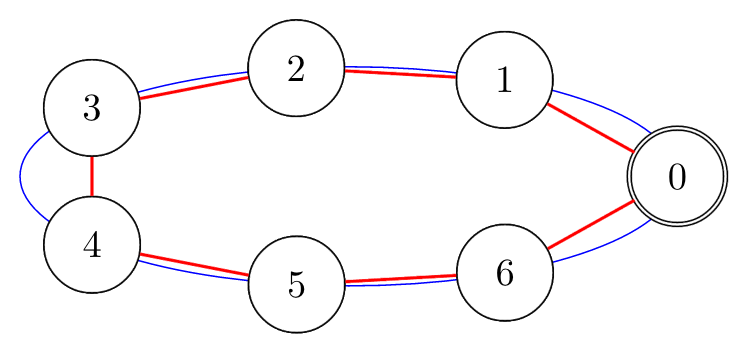
\includegraphics[scale = 0.3]{images/poligono-elipse.png} \hfill}
\end{frame}


\subsection{Rotating calipers}

\begin{frame}{Rotating calipers}
    \begin{itemize}
        \item Caliper en inglés es calibre.
        \item Esto es un calibre:
    \end{itemize}
        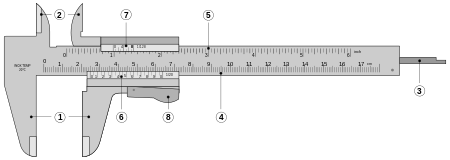
\includegraphics[scale = 0.75]{images/calibre.png}
\end{frame}

\begin{frame}{Rotating calipers (cont)}
    \begin{itemize}
        \item La analogía surge de imaginar que vamos girando un calibre ajustado al polígono todo el tiempo.
        \item Nuestro calibre siempre toca \textbf{dos vértices} del polígono.
        \item Un par de vértices que son tocados al mismo tiempo para alguna rotación del calibre, se llama un par \textbf{antipodal}
        \item El método de rotating calipers consiste en simular eficientemente en $O(N)$ este proceso de rotación, enumerando todos los pares antipodales
        \item Caso borde del recorrido: Si el polígono tiene dos lados paralelos, cuando el calibre se ajusta a ellos hay $4$ pares de vértices antipodales,
               correspondientes a esos dos lados.
    \end{itemize}
\end{frame}

\begin{frame}{Rotating calipers: Algoritmo}
    \begin{itemize}
        \item En nuestro caso, giraremos en sentido \textbf{horario}
        \item De un lado, comenzamos con un vértice $p$ de mínimo $x$, y en caso de empate el de mínimo $y$
        \item Del otro lado comenzamos con un vértice $q$ de máximo $x$, y en caso de empate el de máximo $y$
        \item $(p,q)$ es nuestro primer par antipodal.
        \item En cada paso consideramos los vértices siguientes a $p$ y $q$ en sentido horario, que son $p_n$ y $q_n$
        \item De esos dos, elegimos avanzar por ``el que primero es tocado por los calibres'', cambiando así a:
                \begin{itemize}
                    \item $(p_n, q)$ si $(p_n - p) \times (q_n - q) > 0$
                    \item $(p, q_n)$ si $(p_n - p) \times (q_n - q) < 0$
                    \item Si $(p_n - p) \times (q_n - q) = 0$, $(p, p_n)$ y $(q, q_n)$ son lados paralelos. Los procesamos y avanzamos a $(p_n, q_n)$
                \end{itemize}
    \end{itemize}
\end{frame}


\begin{frame}{Aplicación al problema original}
    \begin{itemize}
        \item Se puede observar que la distancia máxima entre vértices se alcanza necesariamente en un par antipodal.
        \item Con el método de rotating calipers, los enumeramos en $O(N)$ y tomamos el par más lejano encontrado.
    \end{itemize}
\end{frame}


\end{document}
